\subsection{Export data from the PCDB: The SQL-query tool}\label{subsec_sql_query_tool}
While the `Data Viewer' only allows to view data (and to edit data only manually, one-by-one, in case you have writing-rights), \texttt{pgAdmin3}'s SQL-query tool allows to actually write and execute SQL-queries to obtain data from tables and views. 
Moreover, the SQL-Query tool allows to export the result-set of your query (a data table) to a file. 
Using the SQL-query tool is therefore the easiest way to export data from the PCDB.

Figure \ref{fig_pgadmin3_sql_query_tool_editor_country} and \ref{fig_pgadmin3_sql_query_tool_builder_country} show the two ways in which you may query data using the SQL-query tool, again using the example of of the country table in the \texttt{config\_data} schema.
\begin{itemize}
\item[(a)]{You may explicitly write SQL code to define a query in the `SQL Editor' tab of the SQL-query tool window's top panel. Double-clicking the green play-button in the SQL-query tool's toolbar (second from left in figure \ref{fig_pgadmin3_sql_query_tool_toolbar}) will execute the query; the result will be displayed as data table in the `Output pane' (bottom panel of the window).}
\item[(b)]{You may construct your query manually, using the in the `Graphical Query Builder' tab of the SQL-query tool window's top panel. Double-clicking the green play-button in the SQL-query tool's toolbar (second from left in figure \ref{fig_pgadmin3_sql_query_tool_toolbar}) will return the manually built query in explicit SQL code, execute it, and display the result as data table in the `Output pane' (bottom panel of the window).}
\end{itemize}

\begin{figure}[ht!]
\centering
  \begin{subfigure}{.45\textwidth}
  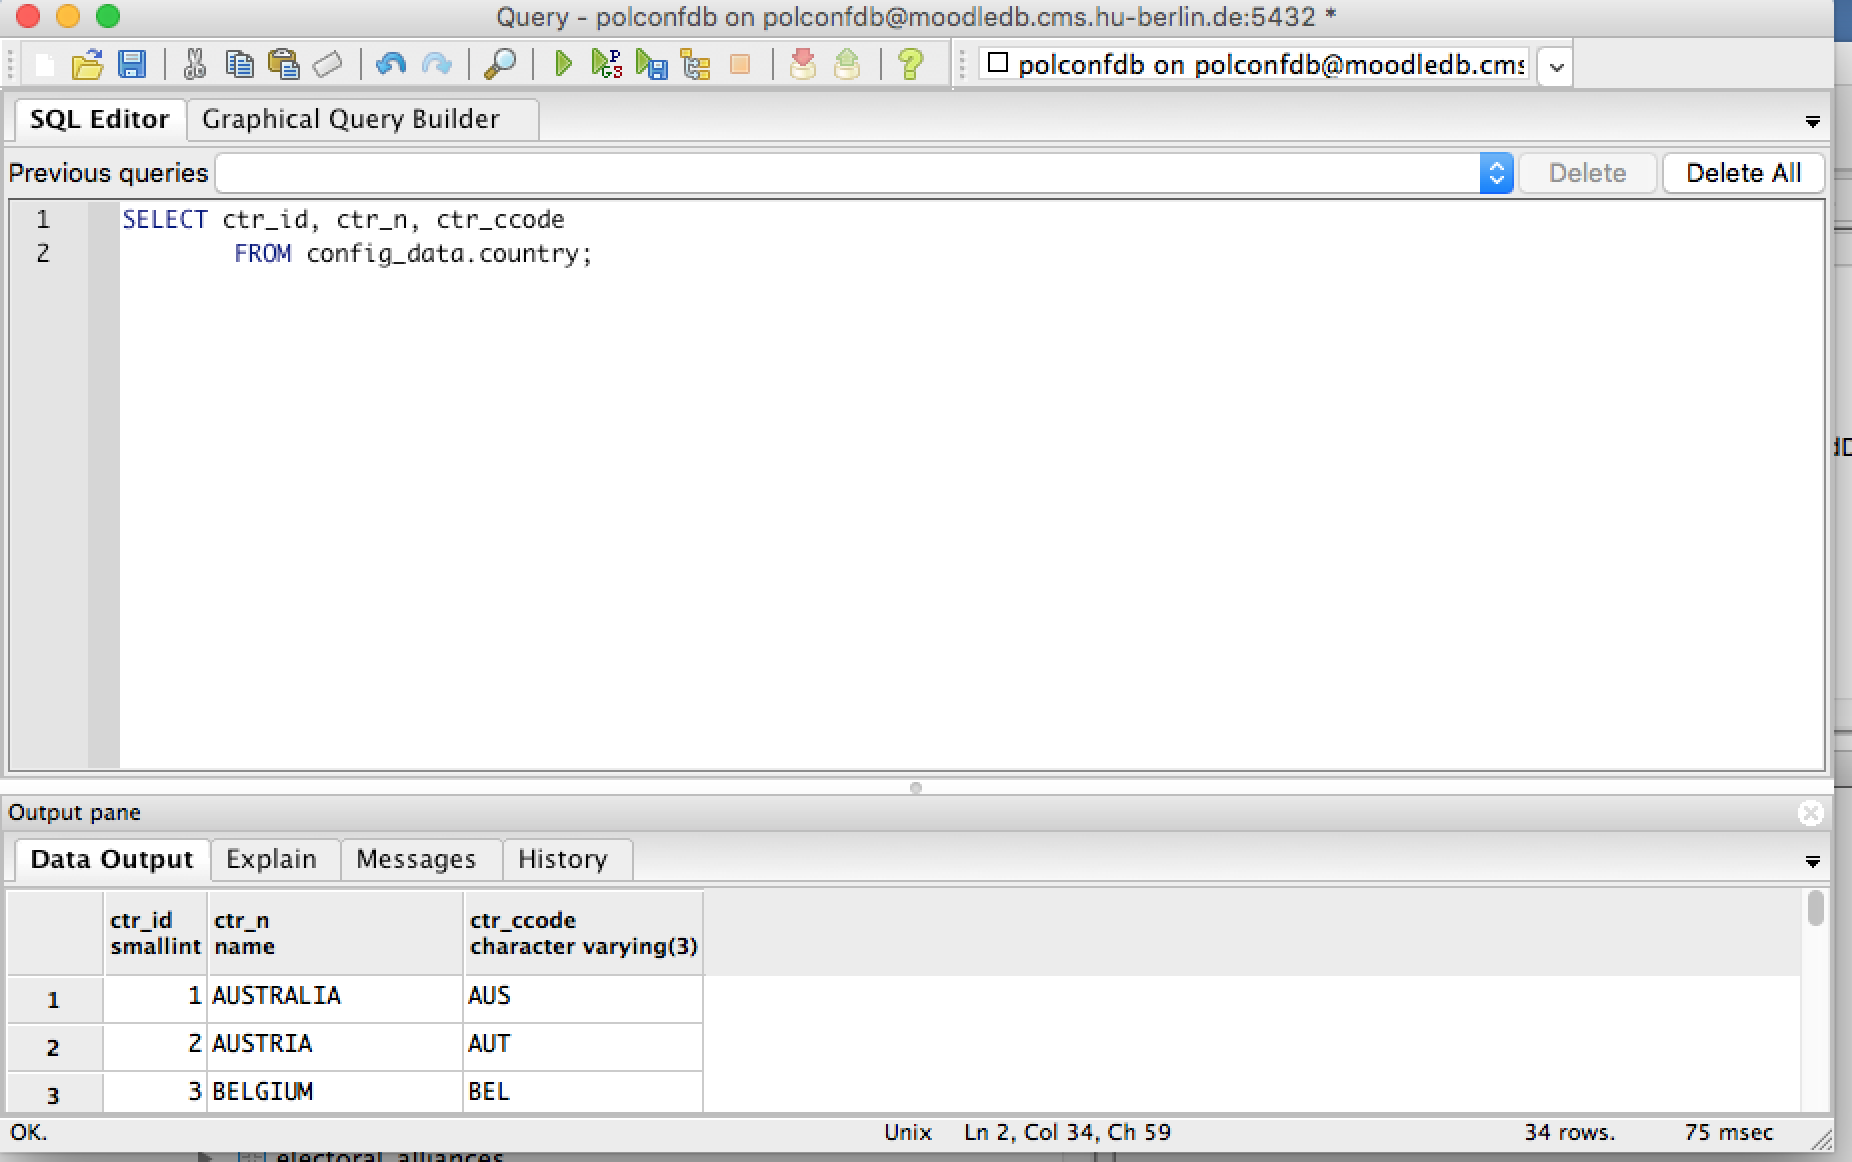
\includegraphics[width=\textwidth,trim= 0 0 0 0, clip]{pcdb_documentation_screenshots/pgadmin3_sql_query_tool_editor_country.png}
    \subcaption{Query data with explicit SQL code from country table in the `SQL Editor' tab.}
    \label{fig_pgadmin3_sql_query_tool_editor_country}
  \end{subfigure}
  ~%
  \begin{subfigure}{.45\textwidth}
  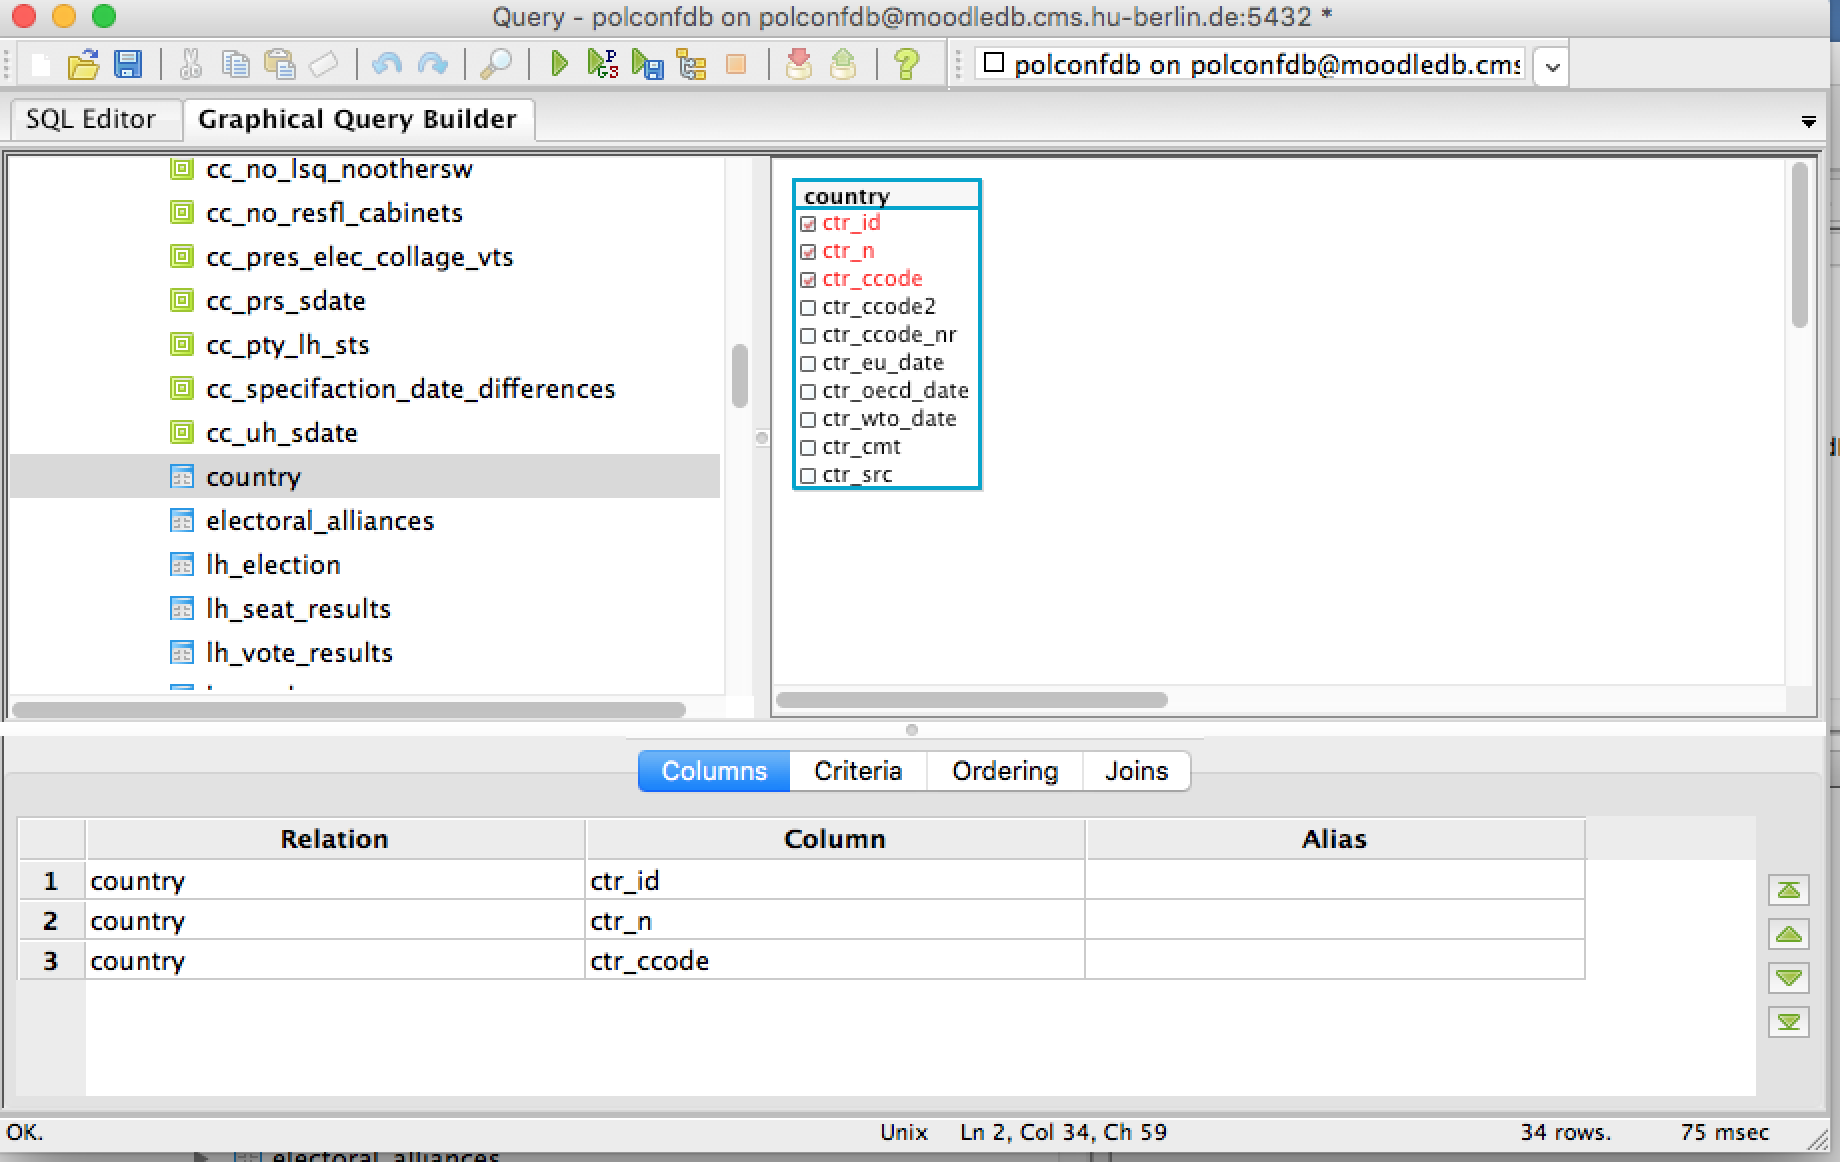
\includegraphics[width=\textwidth,trim= 0 0 0 0, clip]{pcdb_documentation_screenshots/pgadmin3_sql_query_tool_builder_country.png}
    \subcaption{Query data from country table  by manual selection in the `Graphical Query Builder' tab.}
    \label{fig_pgadmin3_sql_query_tool_builder_country}
  \end{subfigure} 
  \caption{Two ways to define queries in \texttt{pgadmin3}'s SQL-query tool window.}
\end{figure}

The double-clicking the green play-button in the SQL-query tool's toolbar (second from left in figure \ref{fig_pgadmin3_sql_query_tool_toolbar}) will execute the query; the result will be displayed as data table in the bottom panof the window.
The square shaped icon is the stop button (most right in figure \ref{fig_pgadmin3_sql_query_tool_toolbar}), which allows to cancel a running query.

\begin{figure}[ht!]
\centering
  
\includegraphics[width=.6\textwidth,trim= 0 0 0 0, clip]{pcdb_documentation_screenshots/pgadmin3_sql_query_tool_toolbar.png}
    \caption{Toolbar of \texttt{pgAdmin3}' SQL-query tool window.}
    \label{fig_pgadmin3_sql_query_tool_toolbar}
\end{figure}

The icon that combines a green play-button with a blue-shaded disc (third from right in figure \ref{fig_pgadmin3_sql_query_tool_toolbar}) will open the `Export data to file' wizard, which allows to write the result-set of a query to a file (see figure \ref{fig_pgadmin3_sql_query_tool_export_data_wizard}.
Select a column separator (default is a semicolon \texttt{;}), a quote character (default is the double qute \texttt{''}), select check-box `Column names' in case you want to include column (i.e., variable) names in the first row of the file, and select a path and file name to write to. Then click the `OK' button to export data to file.   

\begin{figure}[ht!]
\centering
  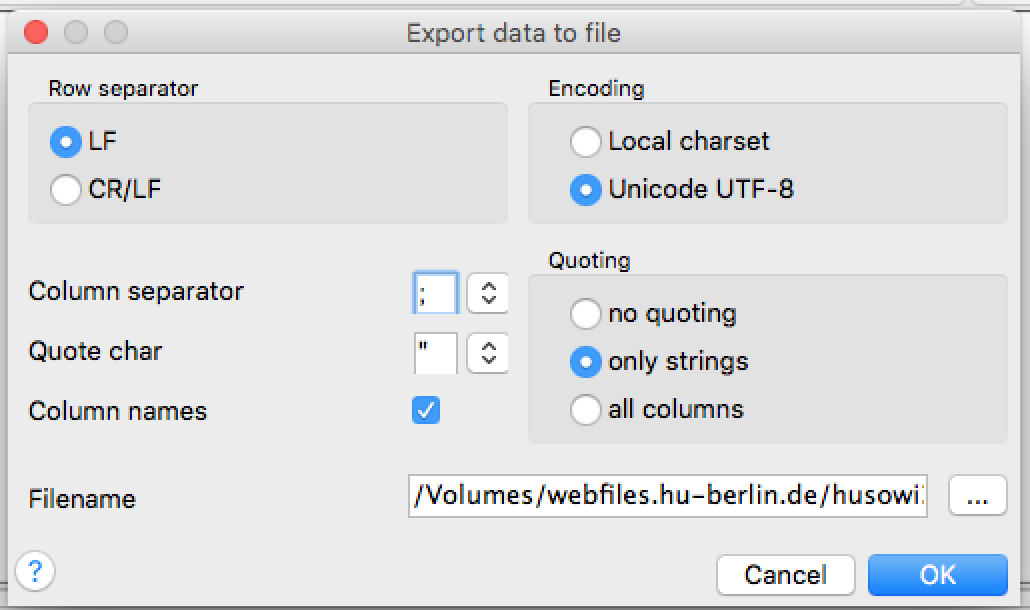
\includegraphics[width=.8\textwidth,trim= 0 0 0 0, clip]{pcdb_documentation_screenshots/pgadmin3_sql_query_tool_export_data_wizard.png}
    \caption{`Export data to file' wizard of \texttt{pgAdmin3}' SQL-query tool.}
    \label{fig_pgadmin3_sql_query_tool_export_data_wizard}
\end{figure}

When saving the result-set of the query to a file in the \texttt{.csv}-format, the result should look familiar to you. It's a plain semicolon-separated table (see figure \ref{fig_pgadmin3_sql_query_tool_export_data_result_example}).

\begin{figure}[ht!]
\centering
  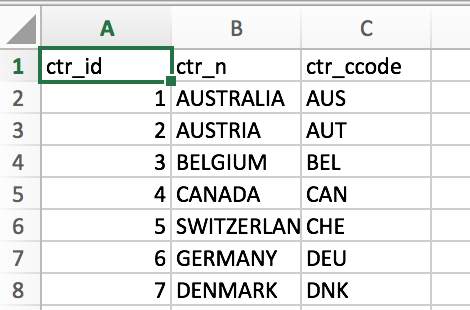
\includegraphics[width=.6\textwidth,trim= 0 0 0 0, clip]{pcdb_documentation_screenshots/pgadmin3_sql_query_tool_export_data_result_example.png}
    \caption{Result after exporting data with \texttt{pgAdmin3}'s `Export data to file' wizard.}
    \label{fig_pgadmin3_sql_query_tool_export_data_result_example}
\end{figure}


